\chapter{Исследовательская часть}

\section{Сравнение результатов затенения}
На рисунках \ref{img:rsm}-\ref{img:fong} представлены результаты
визуализации с использованием различных методов затенения.
Причём была использована одна и та же сцена с одинаковым освещением.
Затухание света с расстоянием до источника не учитывалось.

\begin{figure}[H]
	\centering
	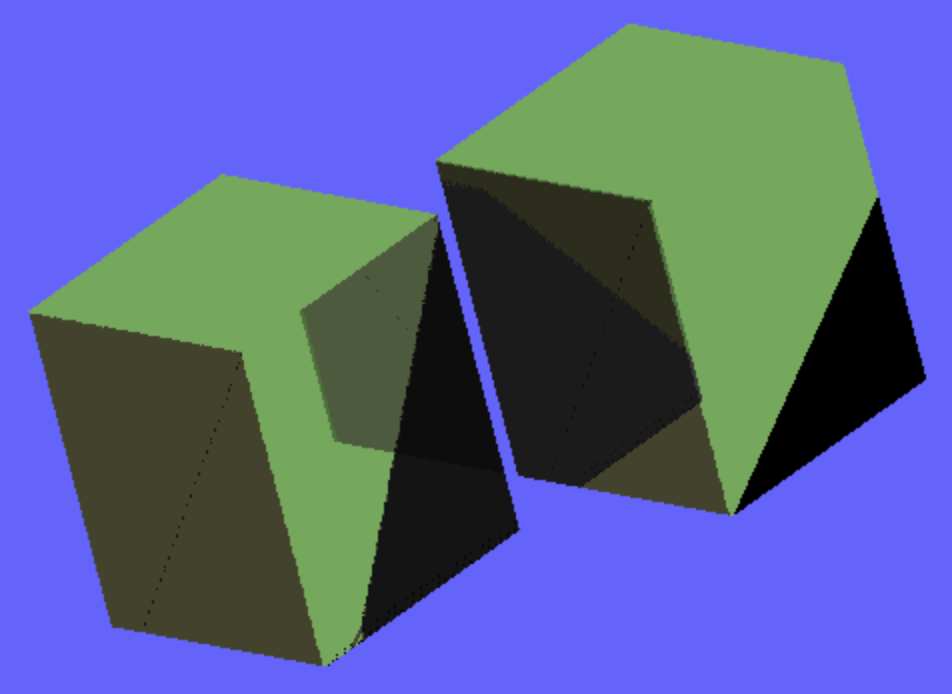
\includegraphics[width=0.8\textwidth]{img/rsm.png}
	\caption{Затенение с помощью отражательной карты теней.}
	\label{img:rsm}
\end{figure}

\begin{figure}[H]
	\centering
	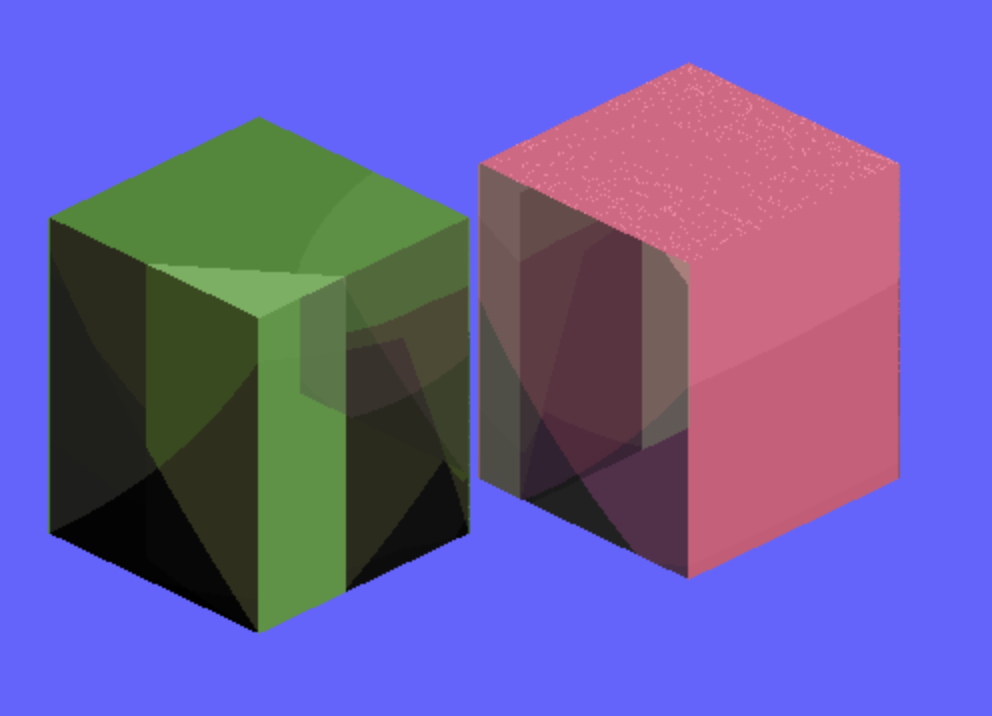
\includegraphics[width=0.8\textwidth]{img/tracing.png}
	\caption{Затенение с помощью трассировки лучей.}
	\label{img:tracing}
\end{figure}

\begin{figure}[H]
	\centering
	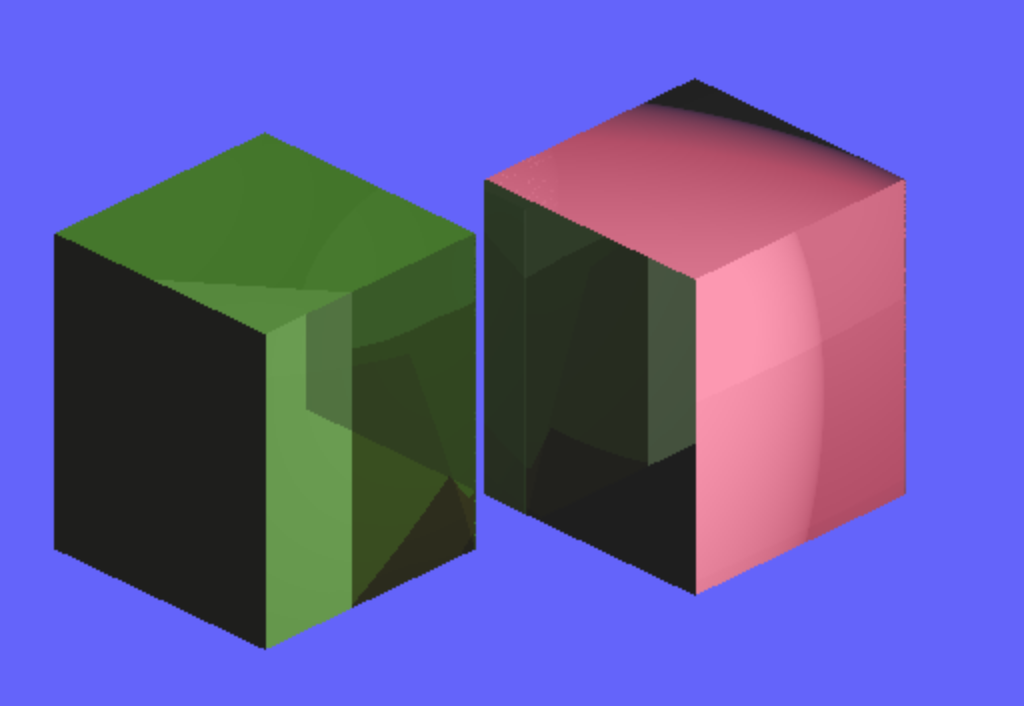
\includegraphics[width=0.8\textwidth]{img/fong.png}
	\caption{Затенение с помощью модели Фонга.}
	\label{img:fong}
\end{figure}

Видно, что реализация алгоритма затенения с помощью отражательной карты теней
дала наибольшую яркость, а с помощью модели Фонга -- наименьшую.
Заметно, что в реализации метода Фонга тени не только
неоднородны, но и могут иметь сильно сглаженные границы.
После прменения карты теней объекты освещены частично,
так как размер буфера источника конечен и некоторые точки проецируются
на плоскость $(xy)$ источника так, что не попадают в расчёт.
Эта проблема может быть решена с помощью добавления источников
света или увеличения размера их буферов.

Представлена таблица 5 с результатами
измерения времени работы алгоритмов в секундах.
Из неё видно, что затенение с помощью трассировки лучей работает
дольше, чем с помощью карты теней.
При расчёте среднего значения использовалось 5 замеров.
При замерах времени ноутбук был включен в сеть электропитания и был нагружен только системными приложениями.

\begin{center}
    \begin{tabular} { |c|c|c|c|c| }
        \hline
        \hspace{0pt} & \multicolumn{4}{|c|}{Шаг} \\
        \hline
        Алгоритм & 8 & 4 & 2 & 1 \\
        \hline
        Карта теней & 0.241 & 0.309 & 0.643 & 1.999 \\
        \hline
        Трассировка & 0.143 & 0.245 & 0.762 & 2.822 \\
        \hline
        Модель Фонга & 0.162 & 0.253 & 0.781 & 2.903 \\
        \hline
    \end{tabular} \\
    \vspace{2mm}
    \small {
        Таблица 5 -- Среднее время генерации кадра при
        использовании разных алгоритмов затенения
        для изображения размером $640 \times 480$ в секундах.
    }
\end{center}


\section*{Выводы}
В результате данного раздела сравнены результаты
3 реализаций методов затенения на примере визуализации сцены.
Также рассчитано среднее время выполнения этих алгоритмов.
